\section{Time-averaged transport by region and initial altitude}
\label{sec:grouped-tamsd}

Before examining directional structure, we ask whether the magnitude of horizontal
transport differs across the three take-off regions and four initial-altitude bands.
These are two separate groupings of the same eligible archive. The regional comparison
uses the Alps, Pyrenees and Channel Coast boxes. The altitude comparison uses every
eligible flight with a finite initial altitude, including flights outside those boxes.
It is therefore not a comparison of four altitude groups within one common region.

The altitude bands retain the names introduced in the dataset chapter:
Plains below \SI{300}{\metre}, Hills from 300 to below \SI{800}{\metre},
Low mountains from 800 to below \SI{1500}{\metre}, and High mountains from
\SI{1500}{\metre} upward. Here the grouping variable is the cleaned trajectory's
GNSS origin altitude, \texttt{alt0}. The earlier exploratory map used the first raw
altitude and allowed a pressure fallback; the present transport grouping uses neither
that fallback nor the instantaneous altitude along the route. These historical labels
do not measure local slope, relief or terrain exposure. A record beginning airborne
can enter a high-altitude band over a low launch region.

\subsection{Flight weighting and the fixed cohort}

The measurement reuses the identified native-grid segment TA-MSDs for all
\num{\StatGroupedParaFlights} paraglider and \num{\StatGroupedHangFlights}
hang-glider flights with eligible segments. Segments contain at least eight fixes
and have native cadence at most \SI{10}{\second}. At each requested lag, the
within-flight average pools all supported displacement origins, and the group
average gives each contributing flight equal weight:
\begin{equation}
 m_f(\tau)=\frac{\sum_s n_{fs}(\tau)m_{fs}(\tau)}{\sum_s n_{fs}(\tau)},\qquad
 M_g(\tau)=\frac{1}{N_g(\tau)}\sum_{f\in g:\,n_f(\tau)>0}m_f(\tau).
 \label{eq:grouped-flight-tamsd}
\end{equation}
This differs from the equal-segment archive average introduced at the beginning
of the chapter. No displacement crosses a segment boundary. For $N_{fs}$ fixes
at interval $\Delta t_{fs}$, the requested lag is rounded to
$k=\operatorname{round}(\tau/\Delta t_{fs})$ native steps and
$n_{fs}=N_{fs}-k$. Stored support requires $1\le k\le\lfloor N_{fs}/2\rfloor$
and $\tau\ge\Delta t_{fs}$. The 59 requested lags span 10--10,000~s; the nearest
one to 1000~s is \SI{\StatGroupedReferenceLagS}{\second}. This grid must not be
relabeled as the exact decade grid used later for PCA and regional differences.

Every curve below keeps only the segments that support the maximum requested lag,
\SI{10000}{\second}, and reuses that same segment and flight set at all 59 lags.
Membership and between-flight weights are therefore independent of $\tau$, which is
what allows curves measured at different lags to be read as one population. The
available origins and the segment weights within a flight still change with lag.
The comparison is conditional on long continuous records. The native rounding rule
can admit slightly different boundary cases from the exact common-grid controls.

For Figs.~\ref{fig:tamsd-regions} and~\ref{fig:tamsd-altitude}, five hundred
complete site--day bootstrap draws are paired across lags within each group.
Shading gives pointwise 95\% percentile intervals; at least 20 contributing groups
and 90\% finite replicates are required. Three paraglider flights have missing cluster keys and
become singleton groups. No missing origin-altitude labels remain in this eligible
population. The bands neither match weather or pilots nor calibrate simultaneous
between-group tests. Displayed curves require at least eight flights, and their
support is shown explicitly.

\subsection{Regional contrasts in the fixed cohort}

\begin{figure}[htbp]
 \centering
 
\includegraphics[width=.94\linewidth]{generated/ch3_tamsd_regions}
 \caption{Horizontal flight TA-MSD by take-off region, separately for the two
 disciplines. Top: squared-displacement mean. Middle: its square root divided
 by the requested lag, the RMS magnitude of the interval-mean ground velocity
 up to native-grid rounding. Bottom: contributing flights, which are constant in
 $\tau$ because every curve retains the same long segments over the full lag range.
 Shading is the pointwise site--day interval. Hang-glider curves for the Pyrenees
 and coast are omitted because the cohort contains only two flights in each;
 their support remains shown.}
 \label{fig:tamsd-regions}
\end{figure}

At \SI{\StatGroupedReferenceLagS}{\second}, the paraglider RMS displacements
$\sqrt{M_g}$ are \SI{\StatGroupedParaAlpsRmsKmFixed}{\kilo\metre} in the Alps,
\SI{\StatGroupedParaPyreneesRmsKmFixed}{\kilo\metre} in the Pyrenees and
\SI{\StatGroupedParaChannelCoastRmsKmFixed}{\kilo\metre} on the coast
(Fig.~\ref{fig:tamsd-regions}), over
\num{\StatGroupedParaAlpsFlightsFixed}, \num{\StatGroupedParaPyreneesFlightsFixed}
and \num{\StatGroupedParaChannelCoastFlightsFixed} flights. The coast leads the two
mountain regions, whose mutual separation is small. These amplitudes belong to the
long-flight cohort, which travels farther at intermediate lags than the archive as
a whole.

The middle panels make a change of scaling easier to see than parallel-looking
log--log curves. A constant $\sqrt{M_g}/\tau$ would correspond to quadratic growth
of this moment. In the fixed cohort the coastal 1000--10,000-s log-slope is
\num{\StatGroupedParaChannelCoastSlopeLongFixed}, against
\num{\StatGroupedParaAlpsSlopeLongFixed} in the Alps and
\num{\StatGroupedParaPyreneesSlopeLongFixed} in the Pyrenees. The coastal curve
stays close to quadratic growth over the last decade while the two mountain regions
fall well below it, and no region exceeds two. These fitted slopes describe separate
ranges of a bending curve; they are not Hurst estimates or calibrated hypothesis tests.

Hang gliders supply no regional comparison in this cohort. Only the Alps retain
enough flights, \num{\StatGroupedHangAlpsFlightsFixed}, giving
\SI{\StatGroupedHangAlpsRmsKmFixed}{\kilo\metre} near the reference lag. The
Pyrenean and coastal groups contain two flights each, below the eight required for
display, so the regional ordering of Fig.~\ref{fig:tamsd-regions} is a paraglider
result alone.

\subsection{Initial-altitude bands and their regional composition}

\begin{figure}[htbp]
 \centering
 
\includegraphics[width=.94\linewidth]{generated/ch3_tamsd_altitude}
 \caption{The same TA-MSD estimators grouped by cleaned GNSS origin altitude.
 The names Plains, Hills, Low mountains and High mountains denote the stated
 altitude bands, not measured terrain classes. All eligible regions enter this
 grouping. Lines, shading and support conventions match Fig.~\ref{fig:tamsd-regions},
 including the fixed cohort.}
 \label{fig:tamsd-altitude}
\end{figure}

The paraglider RMS displacements at the reference lag are
\SI{\StatGroupedParaPlainsRmsKmFixed}{\kilo\metre},
\SI{\StatGroupedParaHillsRmsKmFixed}{\kilo\metre},
\SI{\StatGroupedParaLowMountainsRmsKmFixed}{\kilo\metre} and
\SI{\StatGroupedParaHighMountainsRmsKmFixed}{\kilo\metre}, in increasing
altitude-band order. The two lower bands lie above both mountain-labelled groups,
and the ranking is not monotonic in altitude: High mountains lies above Low
mountains. The long-lag behaviour separates the same way. Over the last decade the
Plains and Hills slopes are \num{\StatGroupedParaPlainsSlopeLongFixed} and
\num{\StatGroupedParaHillsSlopeLongFixed}, against
\num{\StatGroupedParaLowMountainsSlopeLongFixed} and
\num{\StatGroupedParaHighMountainsSlopeLongFixed} in the two mountain bands.

For hang gliders the four bands hold
\num{\StatGroupedHangPlainsFlightsFixed}, \num{\StatGroupedHangHillsFlightsFixed},
\num{\StatGroupedHangLowMountainsFlightsFixed} and
\num{\StatGroupedHangHighMountainsFlightsFixed} flights, giving
\SI{\StatGroupedHangPlainsRmsKmFixed}{\kilo\metre},
\SI{\StatGroupedHangHillsRmsKmFixed}{\kilo\metre},
\SI{\StatGroupedHangLowMountainsRmsKmFixed}{\kilo\metre} and
\SI{\StatGroupedHangHighMountainsRmsKmFixed}{\kilo\metre}. Hills leads and High
mountains trails, so the two disciplines do not share one band ranking. Neither the
band label nor one pooled ranking identifies an effect of altitude on a pilot's
dynamics.

\begin{figure}[htbp]
 \centering
 
\includegraphics[width=\linewidth]{generated/ch3_tamsd_region_altitude}
 \caption{Descriptive cross-classification at the requested
 \SI{\StatGroupedReferenceLagS}{\second} lag, within the same fixed cohort. Each
 cell gives $\sqrt{M_g}$ and its contributing flight count.
 Values with fewer than eight flights are suppressed; counts remain visible.
 The same colour scale applies to both disciplines. These cells carry no
 calibrated intervals and do not standardise task, weather or pilot identity.}
 \label{fig:tamsd-region-altitude}
\end{figure}

Figure~\ref{fig:tamsd-region-altitude} shows why the two groupings are not
independent environmental controls. The coastal cohort is concentrated in Plains,
while Alpine and Pyrenean records mostly occupy the two higher bands. Within the
Alpine paraglider cohort the four band amplitudes lie much closer together than in
the pooled altitude comparison above, and they do not decline with altitude. The
Pyrenees supply only the two mountain bands, whose amplitudes are nearly equal.
The coastal cells above Hills are empty in this cohort, so no general
mountain-versus-coast interpretation follows. For hang gliders only three Alpine
cells survive. Logged origin altitude and regional membership describe selection
as well as possible environmental constraints.

The larger coastal transport amplitude can be compared qualitatively with the
smaller changes of interval-mean velocity measured in
Sec.~\ref{sec:regional-variations}. Greater net progress with smaller velocity
changes is compatible with more persistent advancement and less turning, or an
added mean motion; it does not identify wind as the cause. The native-grid
TA-MSD and the matched-order difference diagnostic use different origins and
nearby, rather than identical, reference lags, so this is not an exact paired
decomposition. A quantitative mechanism test should align those observations and
add independent wind, route, terrain and pilot information.

% TRANSFERRED TO MAIN: original text preserved.
\begingroup\color{red!70!black}
\noindent\textit{Reworked in thesis Section~\ref{sec:fixed-circuit}. Original analysis retained below.}\par
\subsection{Paraglider scaling by altitude and circuit type}
\label{sec:altitude-hurst}

For paragliders, we compare the four altitude bands separately within declared
open and closed circuits, using the task classes of Sec.~\ref{sec:strata-compat}.
Free-distance tasks and distance tasks with one, two or three points form the
open group; triangles, quadrilaterals and out-and-return tasks form the closed
group. This is a catalogue declaration of route type, not a test that a retained
segment returns exactly to its origin. The eligible sample contains
\num{\StatAltitudeHurstOpenFlights} open and
\num{\StatAltitudeHurstClosedFlights} closed flights. The
\num{\StatAltitudeHurstUnknownFlights} flights whose task labels do not identify
either class are excluded from this comparison.

Within each circuit class, we fit all
\num{\StatAltitudeHurstLags} requested lags from
\SI{\StatAltitudeHurstFitLow}{\second} to
\SI{\StatAltitudeHurstFitHigh}{\second}, including both endpoints. For each
circuit class and altitude band, an unweighted least-squares fit in
logarithmic coordinates gives
\begin{equation}
 \log\!\left[\frac{M_g(\tau)}{\SI{1}{\metre\squared}}\right]
 = a_g+\alpha_g\log\!\left[\frac{\tau}{\SI{1}{\second}}\right],
 \qquad H_{\mathrm{eff},g}=\frac{\alpha_g}{2}.
 \label{eq:altitude-effective-hurst}
\end{equation}
This is one fit across the full range, rather than an average of the three
decade slopes. The notation $H_{\mathrm{eff}}$ denotes an effective
second-moment scaling exponent. It does not establish self-similarity,
stationary increments or an intrinsic Hurst parameter for these flights.

\begin{figure}[p]
 \centering
 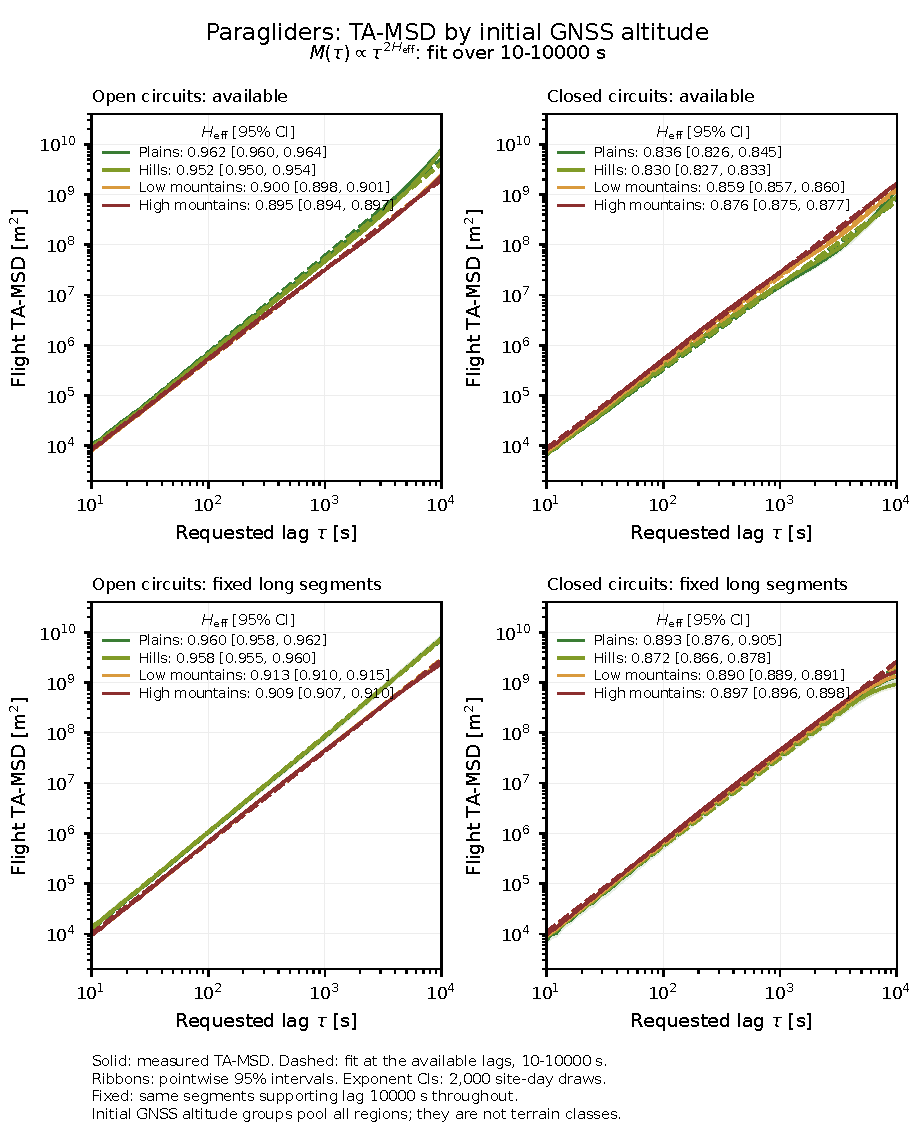
\includegraphics[width=.94\linewidth]{generated/ch3_altitude_hurst}
 \caption{Paraglider horizontal flight TA-MSD by initial GNSS altitude, with
 separate open- and closed-circuit fits over the full 10--10,000-s range.
 Columns distinguish the declared circuit classes. Every panel uses the fixed
 cohort of segments supporting the maximum lag, so flight membership does not
 change with $\tau$. Solid lines show measured means and dashed lines
 the fitted power laws. Legends give $H_{\mathrm{eff}}$ and its marginal 95\%
 site--day bootstrap interval. Ribbons give pointwise 95\% intervals for the
 means. Both use \num{\StatAltitudeHurstResamples} complete cluster draws within
 each circuit--altitude stratum. Flight counts are reported in
 Table~\ref{tab:altitude-hurst}.}
 \label{fig:altitude-hurst}
\end{figure}

Uncertainty is estimated by \num{\StatAltitudeHurstResamples} bootstrap draws
of whole site--day groups within each circuit--altitude stratum. Each draw retains all
flights in every selected group and uses the same cluster multiplicities at
every lag. We recompute the equal-flight mean and
refit Eq.~\eqref{eq:altitude-effective-hurst} on the same lag grid. The 2.5th and
97.5th percentiles of the resulting $H_{\mathrm{eff}}$ values form the reported
interval. This preserves the observed dependence between lags and within a
site--day; it does not treat individual displacement origins or fitted lag
values as independent observations. Every fit has at least twenty contributing
site--day groups at each lag and all
\num{\StatAltitudeHurstResamples} replicates are finite.

\begin{table}[htbp]
 \centering
 \caption{Paraglider effective exponents $H_{\mathrm{eff}}$ from the full
 10--10,000-s fit, separately for declared open and closed circuits.
 Brackets give marginal 95\% site--day bootstrap intervals. Flight counts give the
 fixed cohort, which contributes the same flights at every lag. Weighting matches
 Fig.~\ref{fig:altitude-hurst}.}
 \label{tab:altitude-hurst}
 \small
 % Generated by scripts/esperimenti/ch04_global_transport/generate_altitude_hurst.py
\begin{tabular}{@{}lcc@{}}
\toprule
Altitude band & Fixed cohort & Flights \\
\midrule
\multicolumn{3}{@{}l}{\textit{Open circuits}} \\
\addlinespace[2pt]
Plains & $0.9600\;[0.9577,\,0.9621]$ & $\num{393}$ \\
Hills & $0.9578\;[0.9554,\,0.9600]$ & $\num{417}$ \\
Low mountains & $0.9125\;[0.9103,\,0.9148]$ & $\num{1564}$ \\
High mountains & $0.9088\;[0.9072,\,0.9103]$ & $\num{2209}$ \\
\addlinespace[3pt]
\multicolumn{3}{@{}l}{\textit{Closed circuits}} \\
\addlinespace[2pt]
Plains & $0.8933\;[0.8761,\,0.9054]$ & $\num{24}$ \\
Hills & $0.8720\;[0.8660,\,0.8781]$ & $\num{97}$ \\
Low mountains & $0.8900\;[0.8887,\,0.8914]$ & $\num{3887}$ \\
High mountains & $0.8966\;[0.8956,\,0.8975]$ & $\num{5770}$ \\
\addlinespace[3pt]
\bottomrule
\end{tabular}

\end{table}

Table~\ref{tab:altitude-hurst} and Fig.~\ref{fig:altitude-hurst} separate the
altitude comparison from the mixture of declared task types. Open circuits have
larger fitted exponents than closed circuits in every altitude band. The altitude
ordering also changes with circuit class: for open circuits Plains and Hills lie
about 0.05 above both mountain-labelled groups, whereas the four closed-circuit
exponents fall within 0.025 of one another and follow no altitude order, with High
mountains highest and Hills lowest. Flight support differs substantially between
strata. In particular, the closed-circuit Plains stratum contains only
\num{\StatAltitudeHurstClosedPlainsFixedFlights} flights in
\num{\StatAltitudeHurstClosedPlainsFixedClusters} site--day groups. Its interval
should be read alongside this small population. The cohort conditions on long
continuous records; it does not match the open and closed groups by duration,
region, weather or pilot. Differences between their fitted exponents can therefore
reflect both route geometry and population composition.

These intervals assume independently resampleable site--day groups. Repeated
pilots or weather shared across groups can leave dependence unaccounted for.
They quantify sampling uncertainty conditional on the chosen lag range,
weighting and population, and do not include uncertainty from cleaning,
altitude labels or the adequacy of a power law. In particular, the bending
curves and decade slopes above remain relevant even when the full-range
interval is narrow. The marginal intervals are not simultaneous tests of
differences between altitude bands or circuit classes, and the pooled groups do not isolate a
causal altitude effect. Directional moments are needed next because a scalar
TA-MSD does not describe the orientation of motion.

\FloatBarrier
\FloatBarrier
\endgroup
